\documentclass{beamer}
\usepackage{amsmath,amsthm}
\usetheme{Warsaw}

% Commonly-used stuff
\newcommand{\pr}{\mathbb{P}}
\newcommand{\E}{\mathbb{E}}
\newcommand{\R}{\mathbb{R}}
\newcommand{\N}{\mathbb{N}}
\newcommand{\seqx}{\{x_n\}_{n=0}^\infty}
\newcommand{\seqy}{\{y_n\}_{n=0}^\infty}
\newcommand{\seqa}{\{a_n\}_{n=0}^\infty}
\newcommand{\seqb}{\{b_n\}_{n=0}^\infty}

\newtheoremstyle{normal}
	{3pt}			%space above
	{3pt}			%space below
	{}				%body font
	{\parindent}	%indent amount
	{\itshape}		%theorem head font
	{}				%punctuation after theorem head
	{ }		%space after theorem head
	{}				%theorem head specification(??)
\newtheorem{thm}{Theorem}
\newtheorem*{thm*}{Theorem}
\newtheorem{lem}{Lemma}
\newtheorem*{lem*}{Lemma}

\title{Evolutionary Games on the Lattice}
\author{Andrew Sannier}
\date{March 30, 2012}
\begin{document}

\begin{frame}
\titlepage
\end{frame}

\section{Introduction}
\begin{frame}[c]{What is Game Theory?}
\begin{columns}[c]
  \begin{column}{.5\textwidth}
    \begin{figure}  
      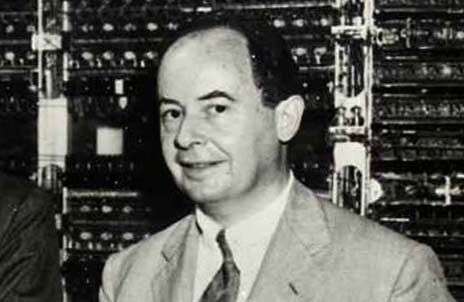
\includegraphics[width=\textwidth]{./images/vonNeumann.jpg}

      \small{John von Neumann}
    \end{figure}
  \end{column}
  \begin{column}{.5\textwidth}
    \begin{figure}
      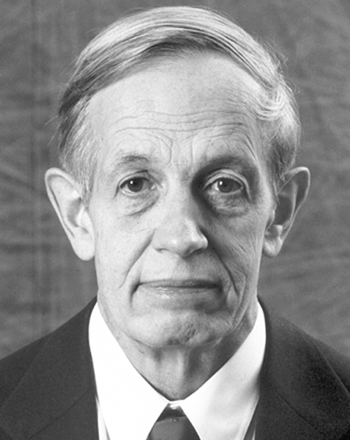
\includegraphics[width=.7\textwidth]{./images/nash.jpg}

      \small{John Nash}
    \end{figure}
  \end{column}
\end{columns}
\begin{block}{}
A set of players assumed to be rational, a set of strategies, and a mapping from strategy to payoff.
\end{block}
\end{frame}

\begin{frame}[c]{The Payoff Matrix}
We encode the mapping from $n$ competing stratgies to player payoff in an $n$-by-$n$ matrix:
\[
    P = 
    \begin{pmatrix}
      a_{11} & a_{12} & \cdots & a_{1n} \\
      a_{21} & & & \\
      \vdots & & \ddots & \\
      a_{n1} & & & a_{nn}
    \end{pmatrix}
\]
\begin{block}{}
  When a player $A$ (using strategy $i$) plays with $B$ (using strategy $j$), $A$ recieves payoff $a_{ij}$ and $B$ receieves $a_{ji}$.
\end{block}
\end{frame}

\begin{frame}[c]{Evolutionary Game Theory}
\begin{columns}[c]
  \begin{column}{0.5\textwidth}
    \begin{figure}
      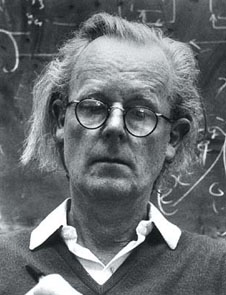
\includegraphics[height=.45\textheight]{./images/maynardSmith.jpg}

      John Maynard Smith
    \end{figure}
  \end{column}
  \begin{column}{0.5\textwidth}
    \emph{Classes of strategies:}

    Strategy $i$ is selfish if $a_{ii} > a_{ji}$ for $j\neq i$. It is altruistic if $a_{ii} < a_{ji}$ for $j\neq i$.
  \end{column}
\end{columns}
\begin{block}{}
  No rationality assumption; players have fixed strategies.
  
  Models an evolutionary system; players interpreted as, for example, types of creatures.
\end{block}
\end{frame}

% \begin{frame}[c]{Types of games in EGT}
% \begin{figure}
%   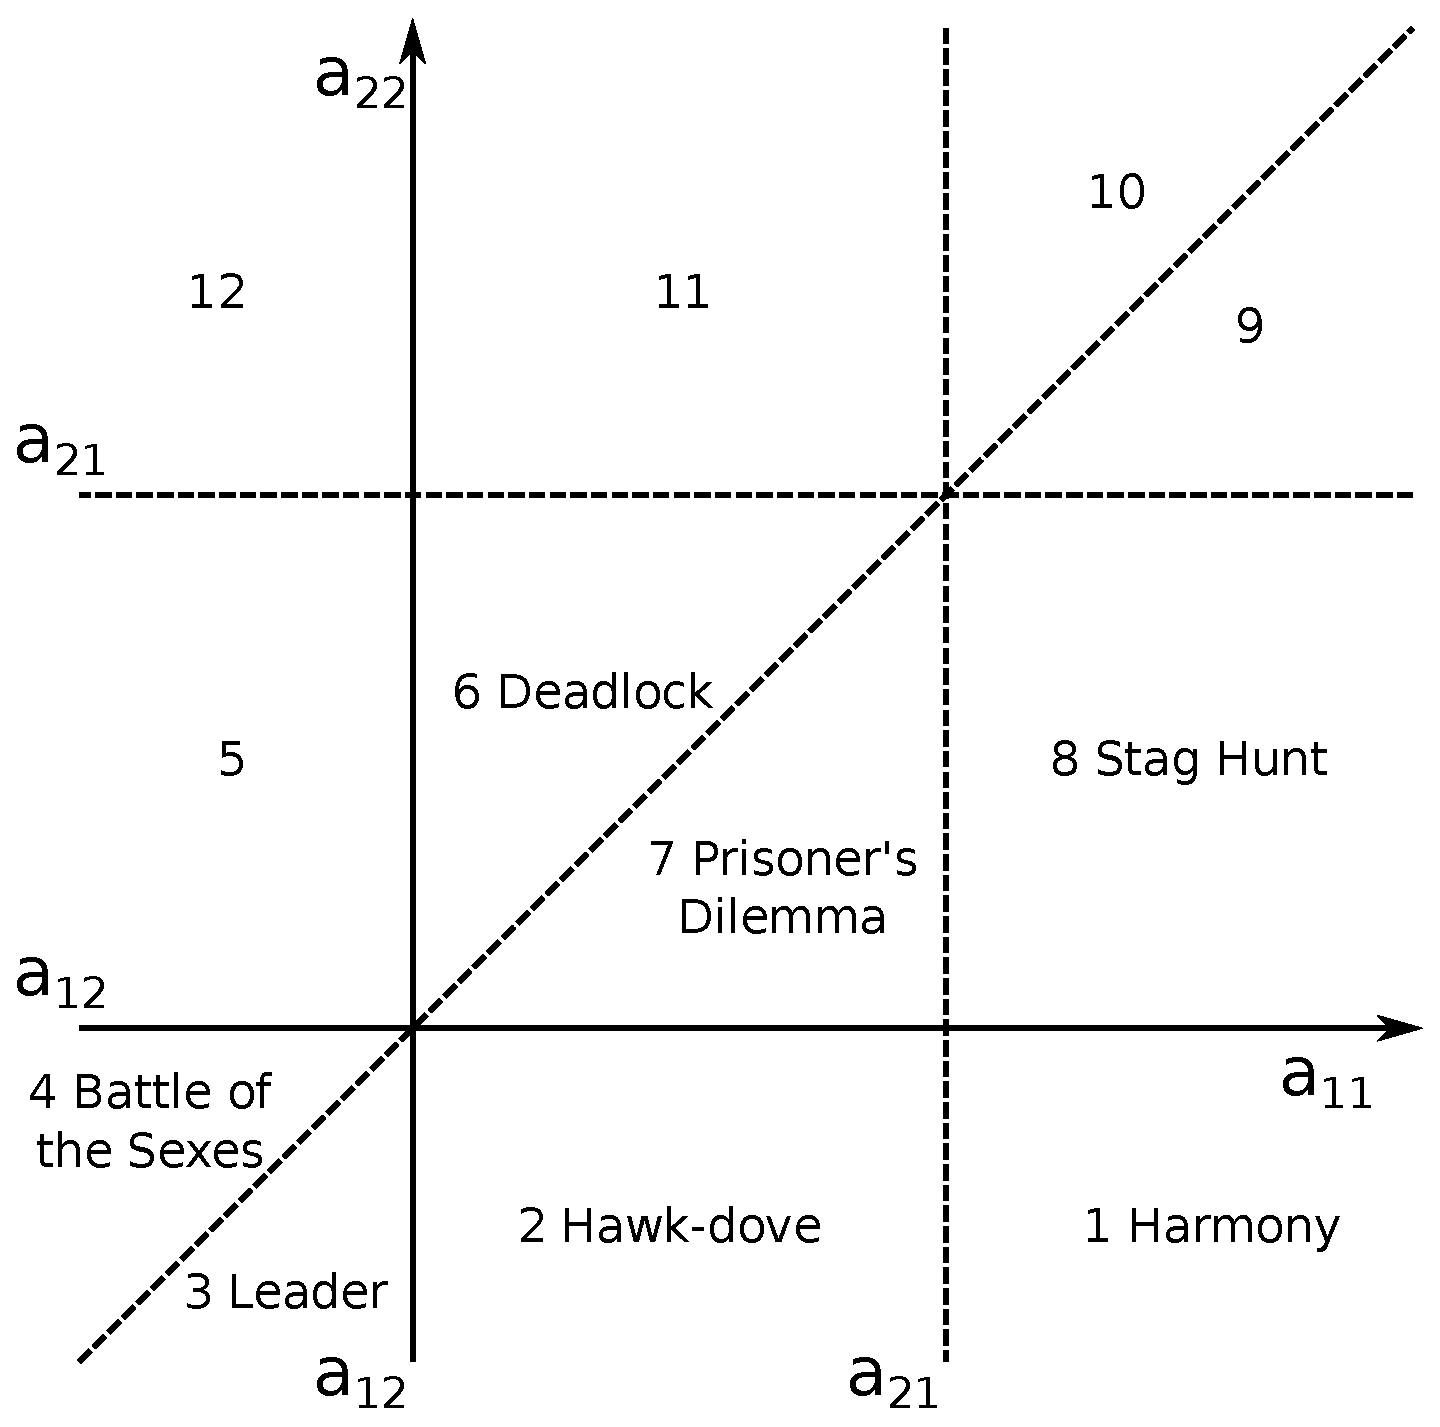
\includegraphics[width=.5\textwidth]{./images/types_of_games_plot.eps}
% \end{figure}
% \begin{block}{}
%   The nature of a game is determined by the order of the payoff coefficients.
% \end{block}
% \end{frame}

\section{A Novel Model}
\begin{frame}[c]{A model with space and stochasticity}
Countably many players on a $d$-dimensional infinite lattice.

Players employ one of $n$ strategies from the set $S = \{1,...,n\}$. 

$\eta_t:\mathbb{Z}^d \to S$ gives the state of the process at time $t$.

Let $\sim$ be a relation on $\mathbb{Z}^d$ such that $\{y: y\sim x\}$ is the set of neighbors of $x$.

$N_i:\mathbb{Z}^d\times \mathbb{R}^+\to \mathbb{Z}^+$ such that
$N_i(x,t) = |\{y\sim x:\eta_t(y) = i\}|$.

We also define an $n$-by-$n$ payoff matrix $P$ as before.

$\phi:\mathbb{Z}^d\times S^{\mathbb{Z}^d} \to \mathbb{R}$ such that
$\phi(x,\eta_t) = \sum_{i=1}^n N_i(x,t)a_{\eta_t(x)i}$.
\end{frame}

\begin{frame}[c]{The infinite lattice}
\begin{figure}
  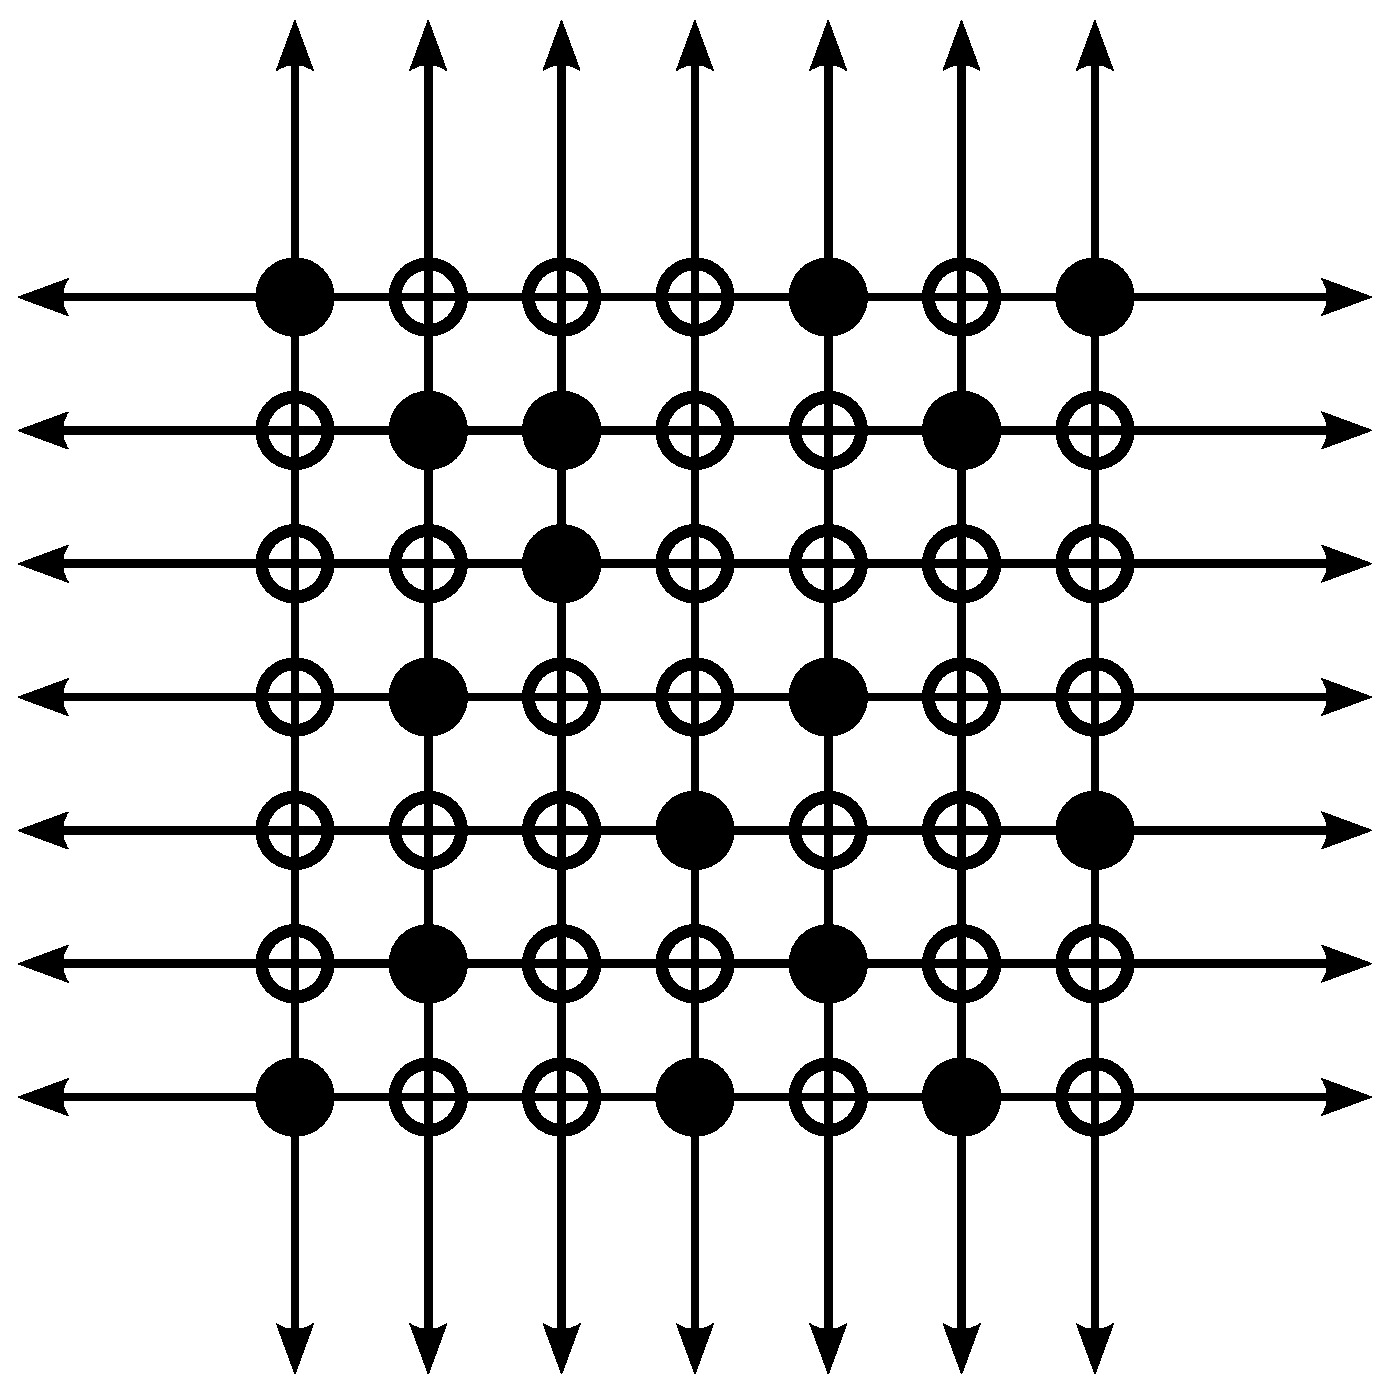
\includegraphics[width=.4\textwidth]{./images/infinite_lattice.eps}
\end{figure}
\begin{block}{}
  \small{We imagine a lattice of sites in $d$-dimensions ($d=2$ above). Each site is home to one player. In this image, players have either a white or black strategy.}
\end{block}
\end{frame}

\begin{frame}[c]{Evolution of the processes}
\emph{Process 1a: Payoff affecting birth and death.}

The player at each site $x$ gives birth at rate $\phi(x,\eta_t)$ if
$\phi(x,\eta_t) > 0$ and dies at rate $-\phi(x,\eta_t)$ if $\phi(x,\eta_t) <
0$. 

Let $y$ be a site chosen uniformly at random from $\{y':y'\sim
x\}$. 

When the player at $x$ gives birth, $\eta_t(y) :=
\eta_t(x)$. 

When the player $x$ dies, $\eta_t(x) := \eta_t(y)$.

\begin{block}{}
  In my thesis, I examine six other ways in which sites can change, but this is the most general.
\end{block}
\end{frame}

\begin{frame}{Standard EGT analysis: An ODE}
\begin{columns}[c]
  \begin{column}{0.4\textwidth}
    Let $X_i$ be the proportion of strategy $i$. 

Then $\phi_i(\vec{X}) = \phi_i(X_1,X_2) = \sum_{j=1}^n a_{ij}X_j$.

In the above process,
\[
    \frac{dX_1}{dt} = X_1X_2\left(\phi_1(\vec{X})-\phi_2(\vec{X})\right).
\]
  \end{column}
  \begin{column}{0.6\textwidth}
\begin{figure}
  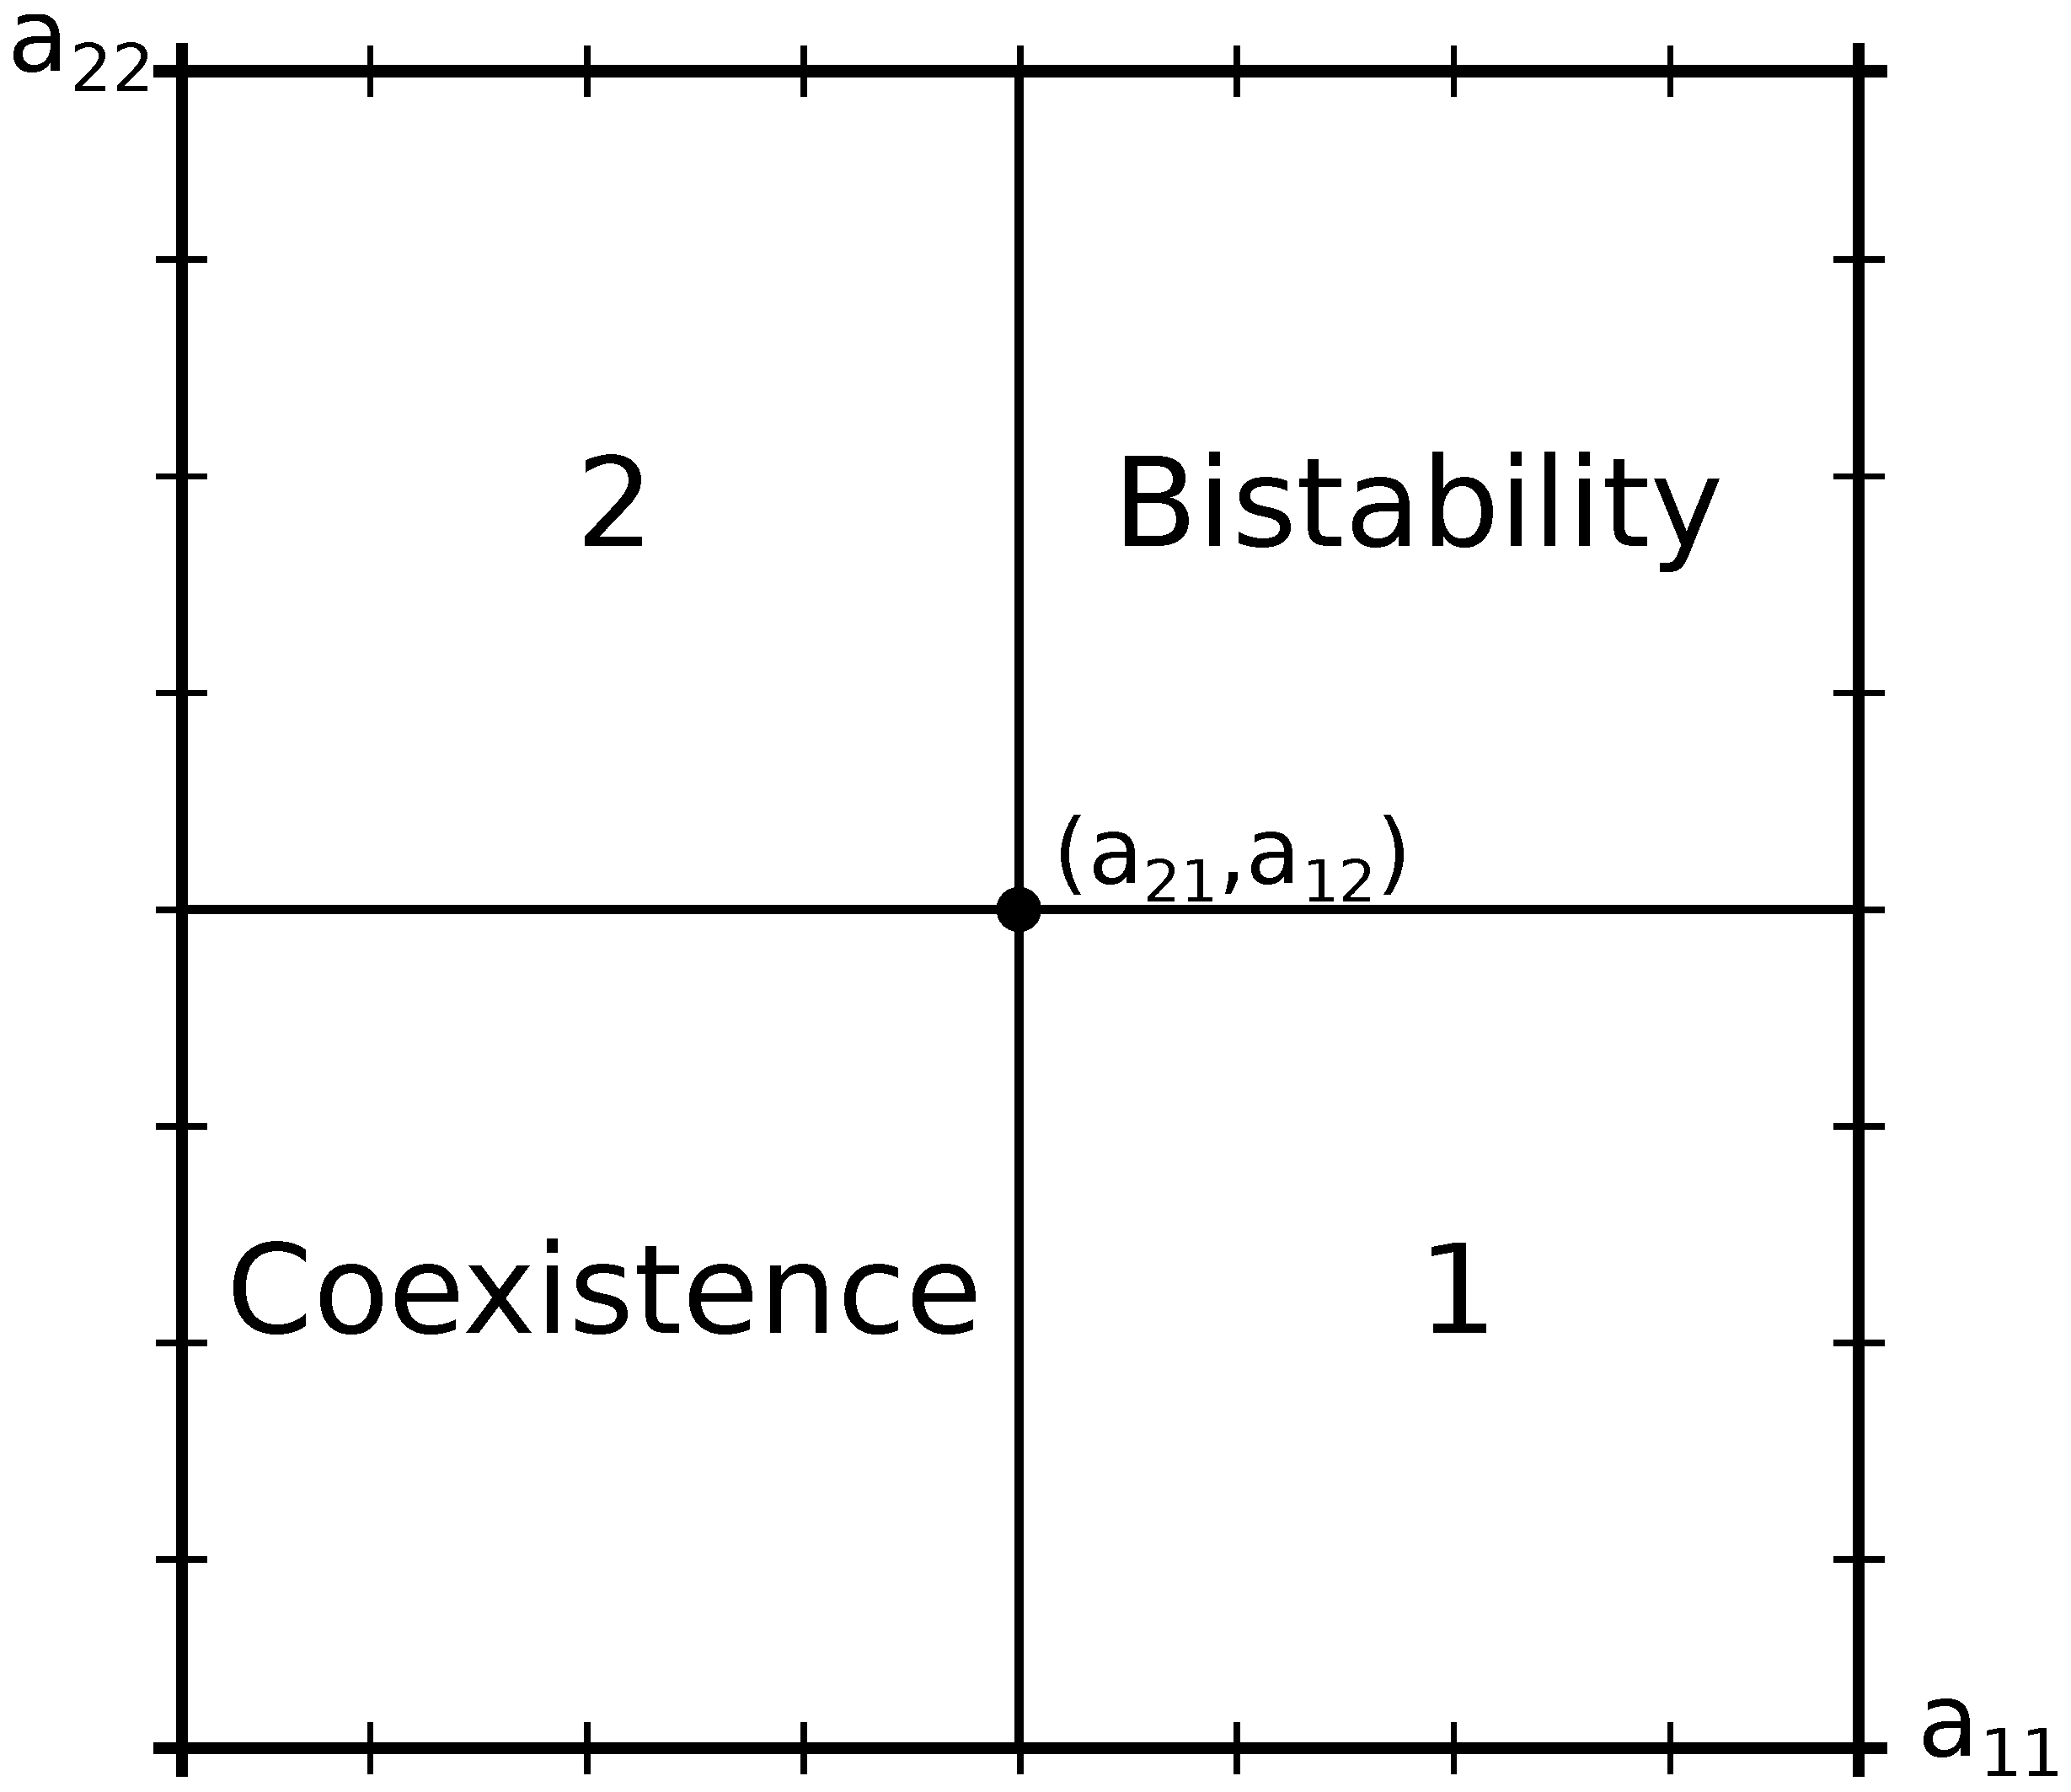
\includegraphics[width=0.8\textwidth]{./images/replicator_bifurcation_diagram.eps}
\end{figure}
  \end{column}
\end{columns}
\begin{block}{}
A mean-field model is constructed by assuming that the players are well-mixing. This mean-field model yields an ODE called the replicator equation.
\end{block}
\end{frame}
\section{Simulation}

\begin{frame}[c]{Simulator in Java}
\begin{figure}
  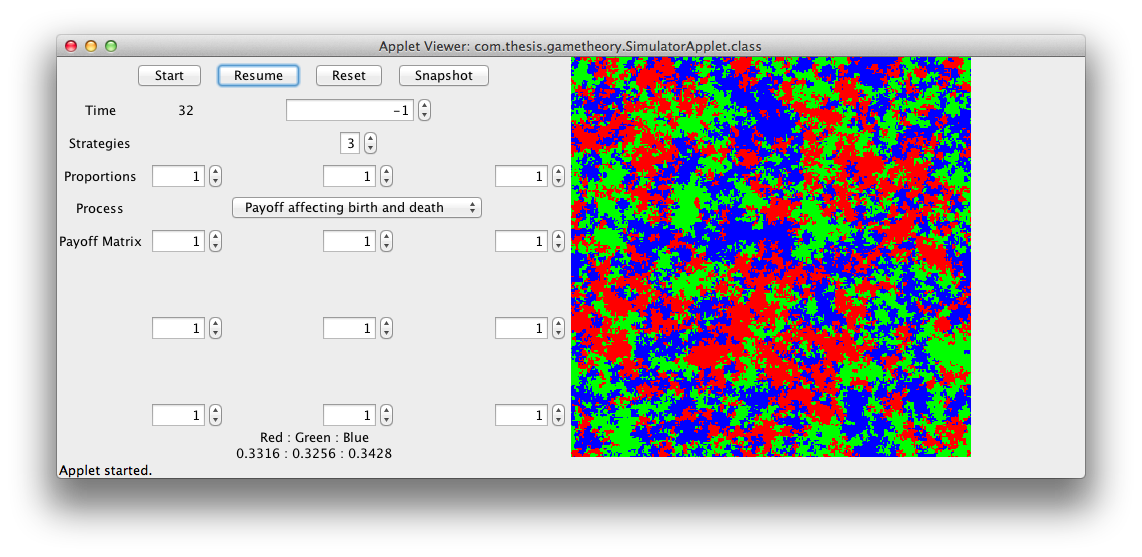
\includegraphics[width=0.83\textwidth]{./images/simulator_screenshot.png}
\end{figure}
\begin{block}{}
  \small{Java application for simulation of these processes. On the right, we see a 400-by-400 lattice after 32 units of time with a 3-by-3 payoff matrix of all 1's.}
\end{block}
\end{frame}

\begin{frame}{Simulating an infinite lattice}
\begin{figure}
  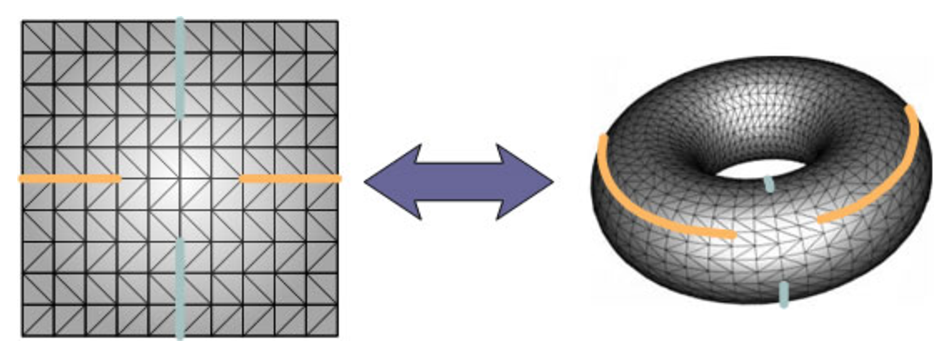
\includegraphics[width=.8\textwidth]{./images/torus.eps}
\end{figure}
\begin{block}{}
  We can't simulate an infinite lattice, so we use periodic boundary conditions to ensure that each site has four nearest neighbors.
\end{block}
\end{frame}

\begin{frame}{A necessary result}
\begin{lem}
  If $T_1,\dots, T_n$ is a collection of $n$ independent exponential
  random variables with rate parameters $\lambda_1,\dots, \lambda_n$,
  then $\pr\left( T_i = \min\{T_1,\dots, T_n\} \right) = \frac{\lambda_i}{\sum_{j=1}^n\lambda_j}$.
\end{lem}

\begin{block}{}
Therefore, each site is equally likely to be the next to update, so we can select a site uniformly at random and then update it.
\end{block}
\end{frame}

\section{Results}
\begin{frame}{Domination, Coexistence, and Clustering}
\begin{columns}[c]
  \begin{column}{0.5\textwidth}
    Domination: one strategy occupies the whole lattice.

    Coexistence: Both strategies present and spatial correlations weak.
\[
    \lim_{t\to\infty} \pr\left(\eta_t(x) \neq \eta_t(y)\right) = 0,\; \forall x,y\in\mathbb{Z}^d,
\]

    Clustering: Both strategies present in distinct clusters.
\[
    \lim_{t\to\infty} \pr\left(\eta_t(x)\neq\eta_t(y)\right) > 0,\; \forall x,y\in\mathbb{Z}^d,
\]
  \end{column}
  \begin{column}{0.6\textwidth}
    \begin{figure}
      
\includegraphics[width=0.5\textwidth]{./images/Time1000-Process0.png}

      
\includegraphics[width=0.5\textwidth]{./images/Time200-Process0.png}
    \end{figure}
  \end{column}
\end{columns}
\end{frame}

\begin{frame}{Departures from the mean-field model}
  \begin{figure}
    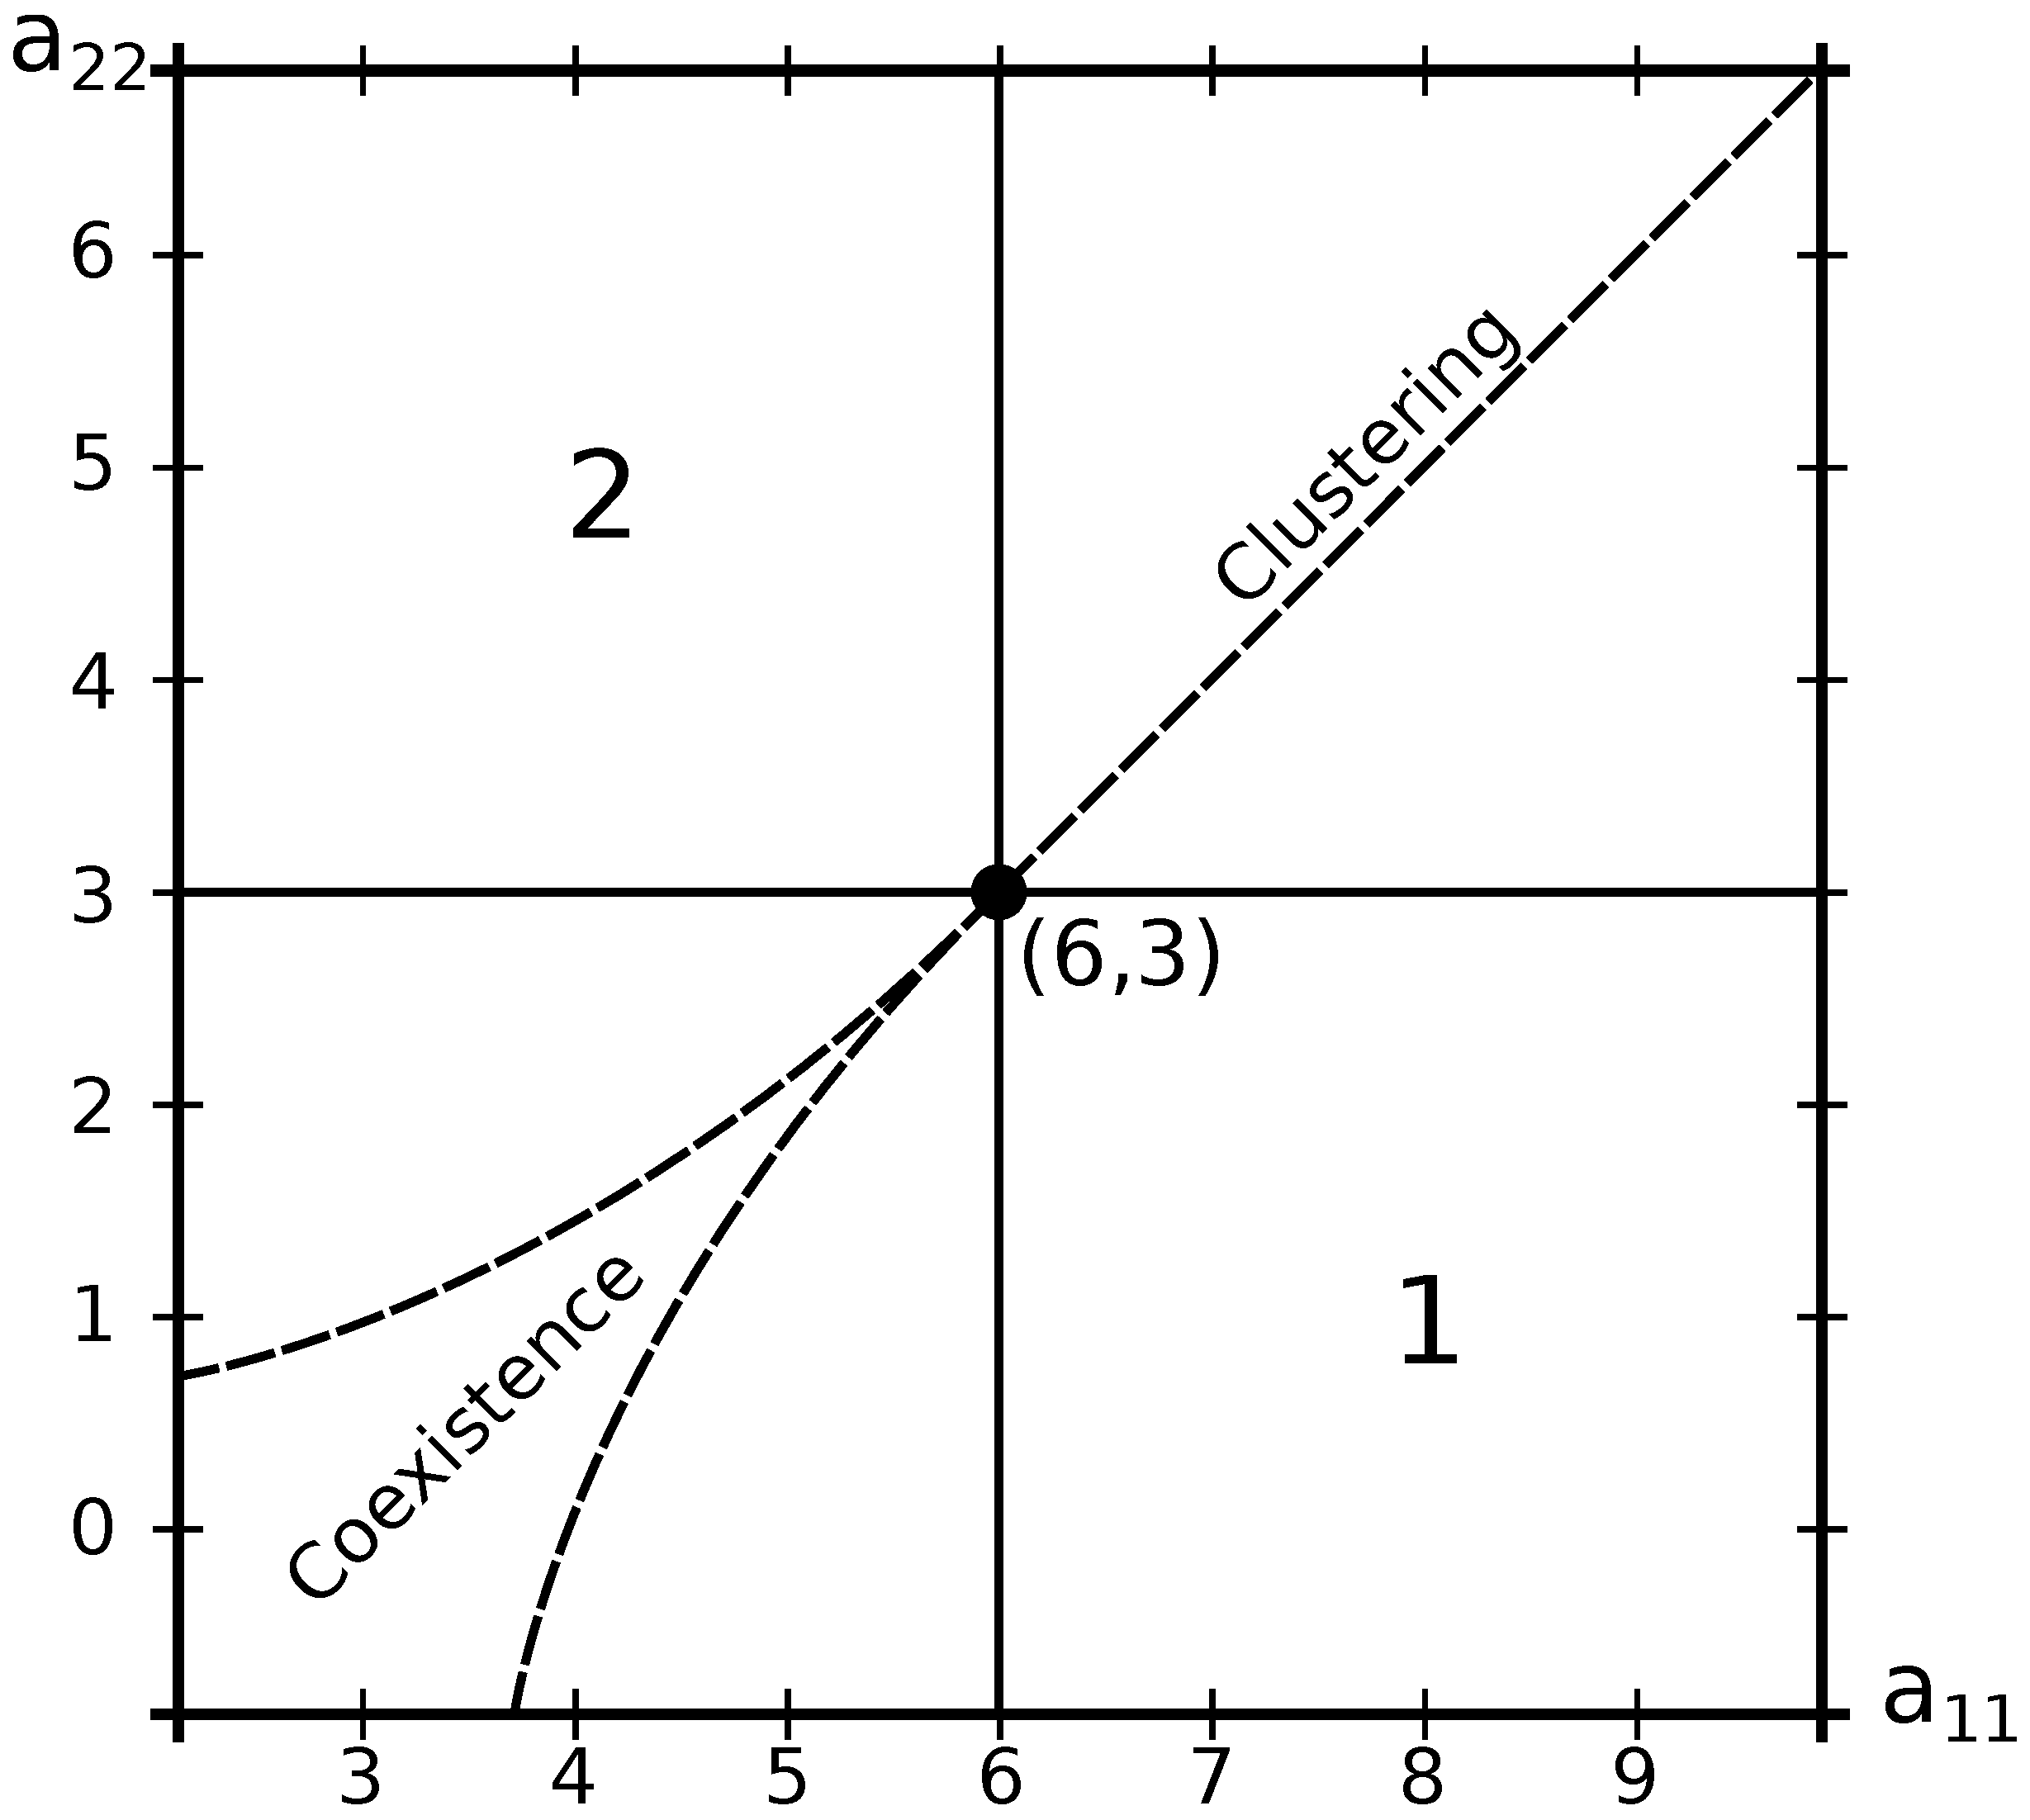
\includegraphics[width=0.33\textwidth]{./images/group_1_bifurcation_diagram.eps}
    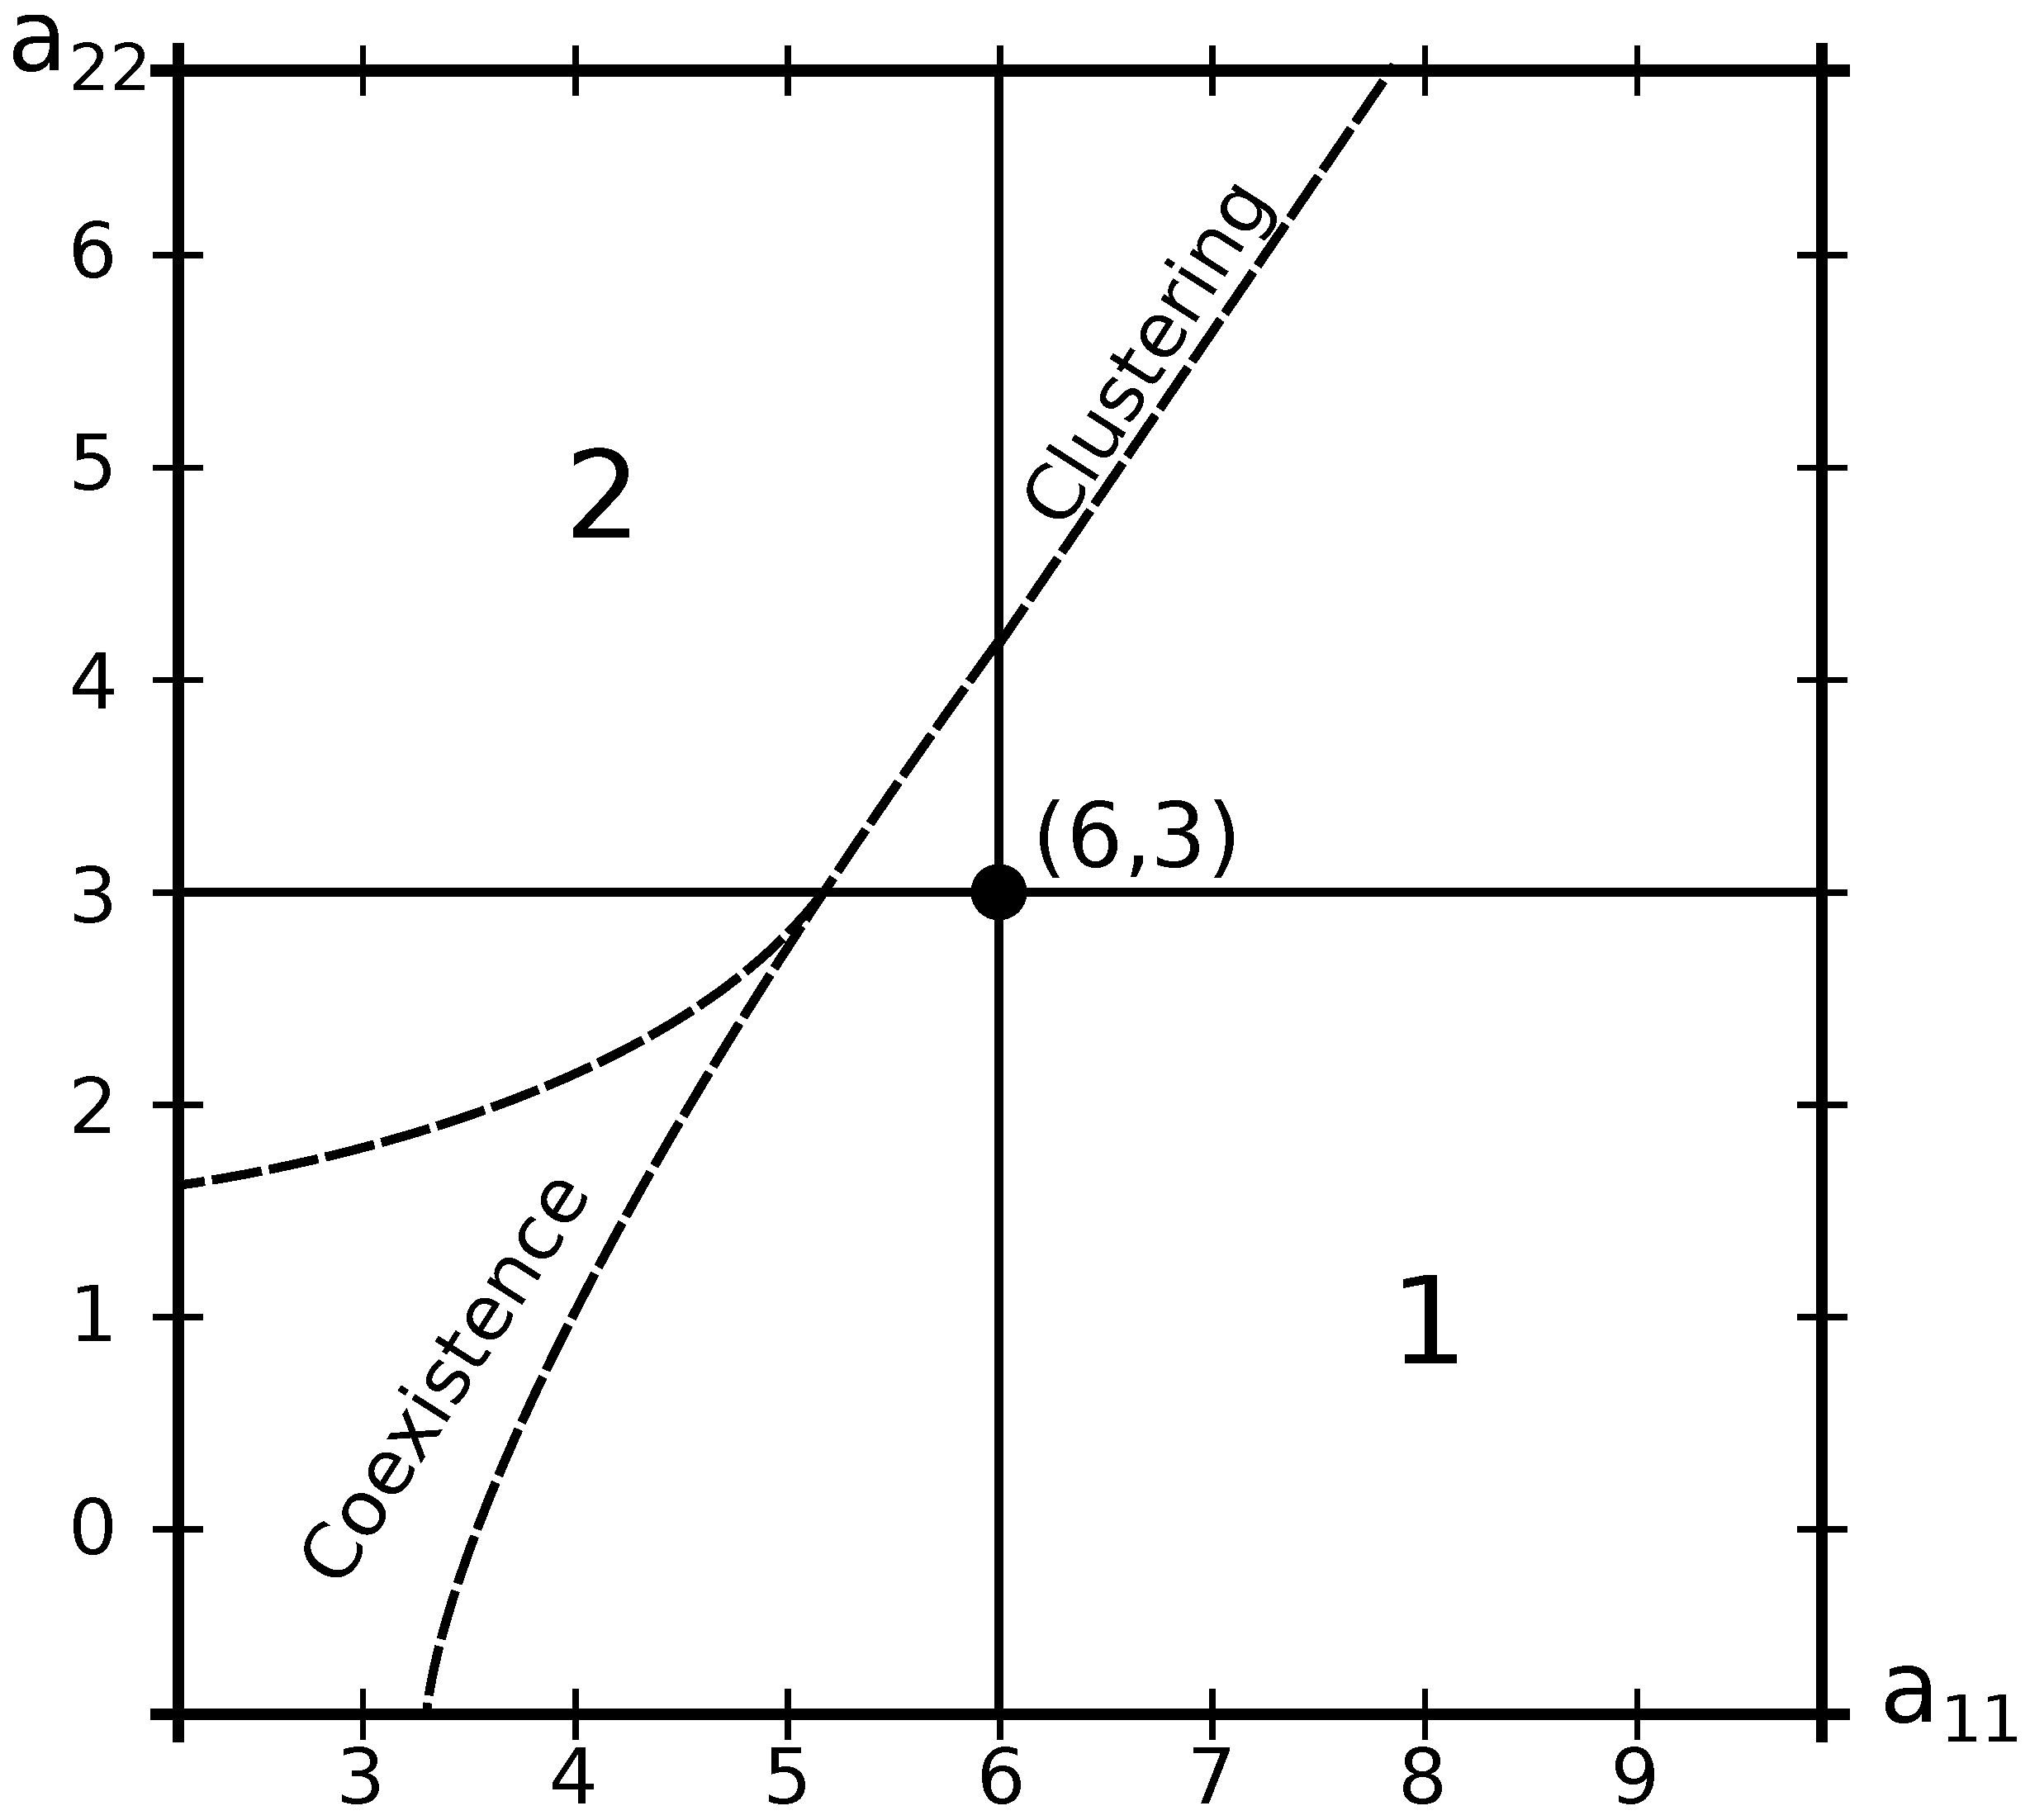
\includegraphics[width=0.33\textwidth]{./images/group_2_bifurcation_diagram.eps}
    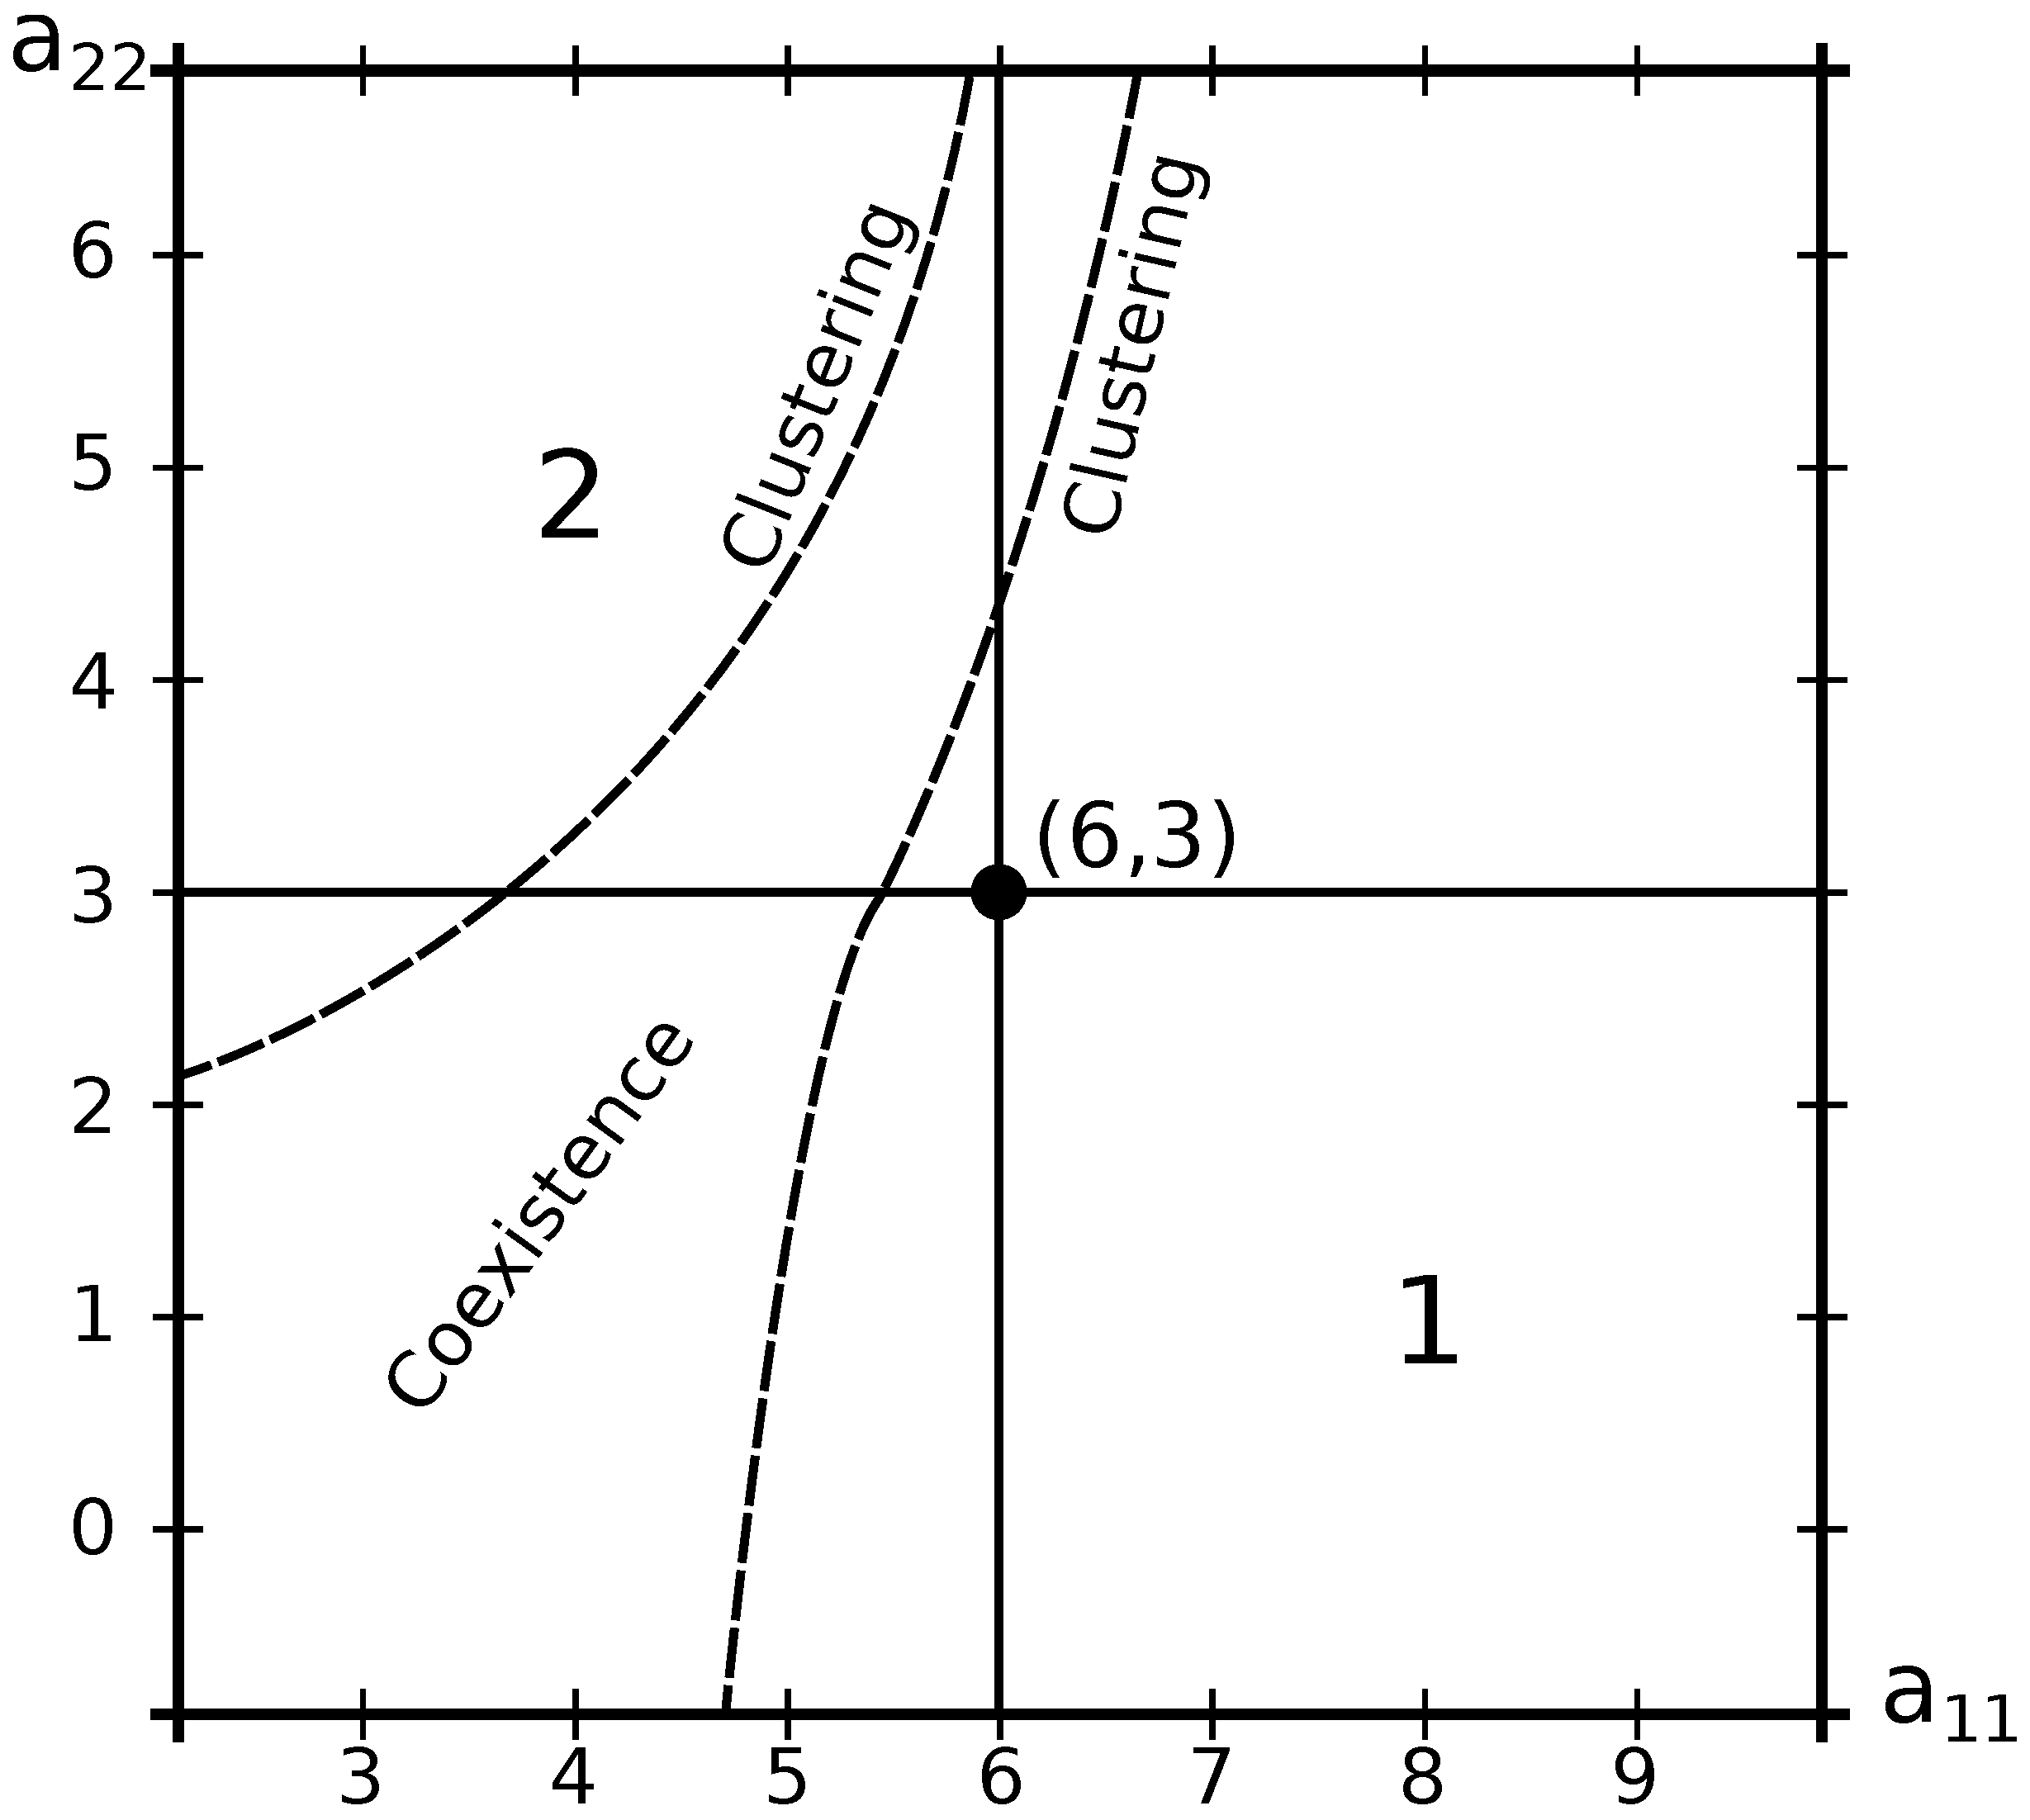
\includegraphics[width=0.33\textwidth]{./images/group_3_bifurcation_diagram.eps}
  \end{figure}
\begin{block}{}
  \small{Bifurcation diagrams from simulation for three significant spatial processes. Payoff matrices along the dotted lines result in clustering, while matrices in the regions between dotted lines result in coexistence.}
\end{block}
\end{frame}

\begin{frame}{Selfishness and hatred}
\begin{figure}
  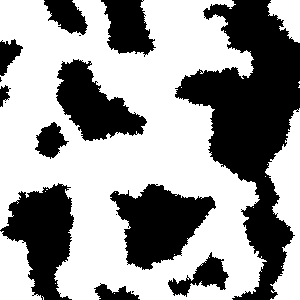
\includegraphics[width=0.4\textwidth]{./images/Time200-Process0-1.png}
  \quad\vline\quad
  
\includegraphics[width=0.4\textwidth]{./images/Time200-Process0.png}
\end{figure}
\begin{block}{}
  Both stills are from simulation with two selfish strategies. In the first, $a_{ij}=0$ for all $i\neq j$; in the second, $a_{ij}=-1$. for all $i\neq j$.
\end{block}
\end{frame}

\begin{frame}{Percolation}
\begin{figure}[h]
  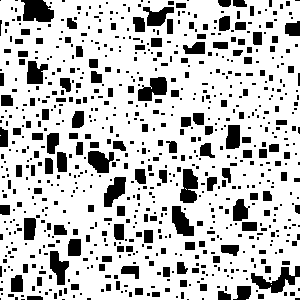
\includegraphics[width=.22\textwidth]{./images/Time4-Process7.png}\quad
  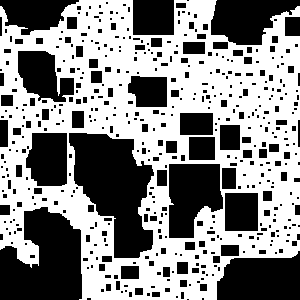
\includegraphics[width=.22\textwidth]{./images/Time25-Process7.png}\quad
  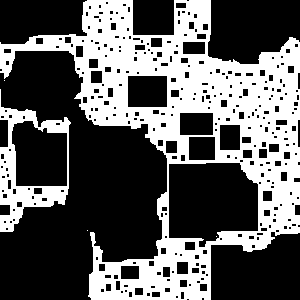
\includegraphics[width=.22\textwidth]{./images/Time41-Process7.png}

  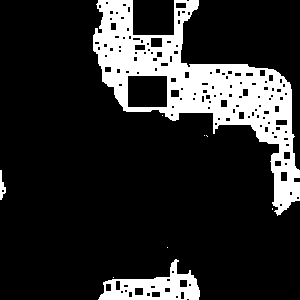
\includegraphics[width=.22\textwidth]{./images/Time61-Process7.png}\quad
  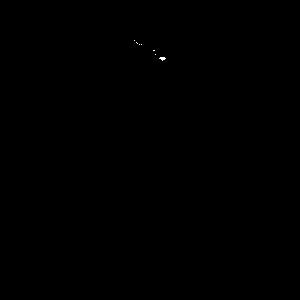
\includegraphics[width=.22\textwidth]{./images/Time95-Process7.png}
\end{figure}
\begin{block}{}
  \small{In this process, each site picks the best possible strategy at each time. The advantage of the black strategy is minimal, but the initial distribution is low enough that it takes some time for domination to occur.}
\end{block}
\end{frame}

\begin{frame}{Cooperation in the prisoner's dilemma}
\begin{columns}[c]
  \begin{column}{0.5\textwidth}
    \begin{figure}
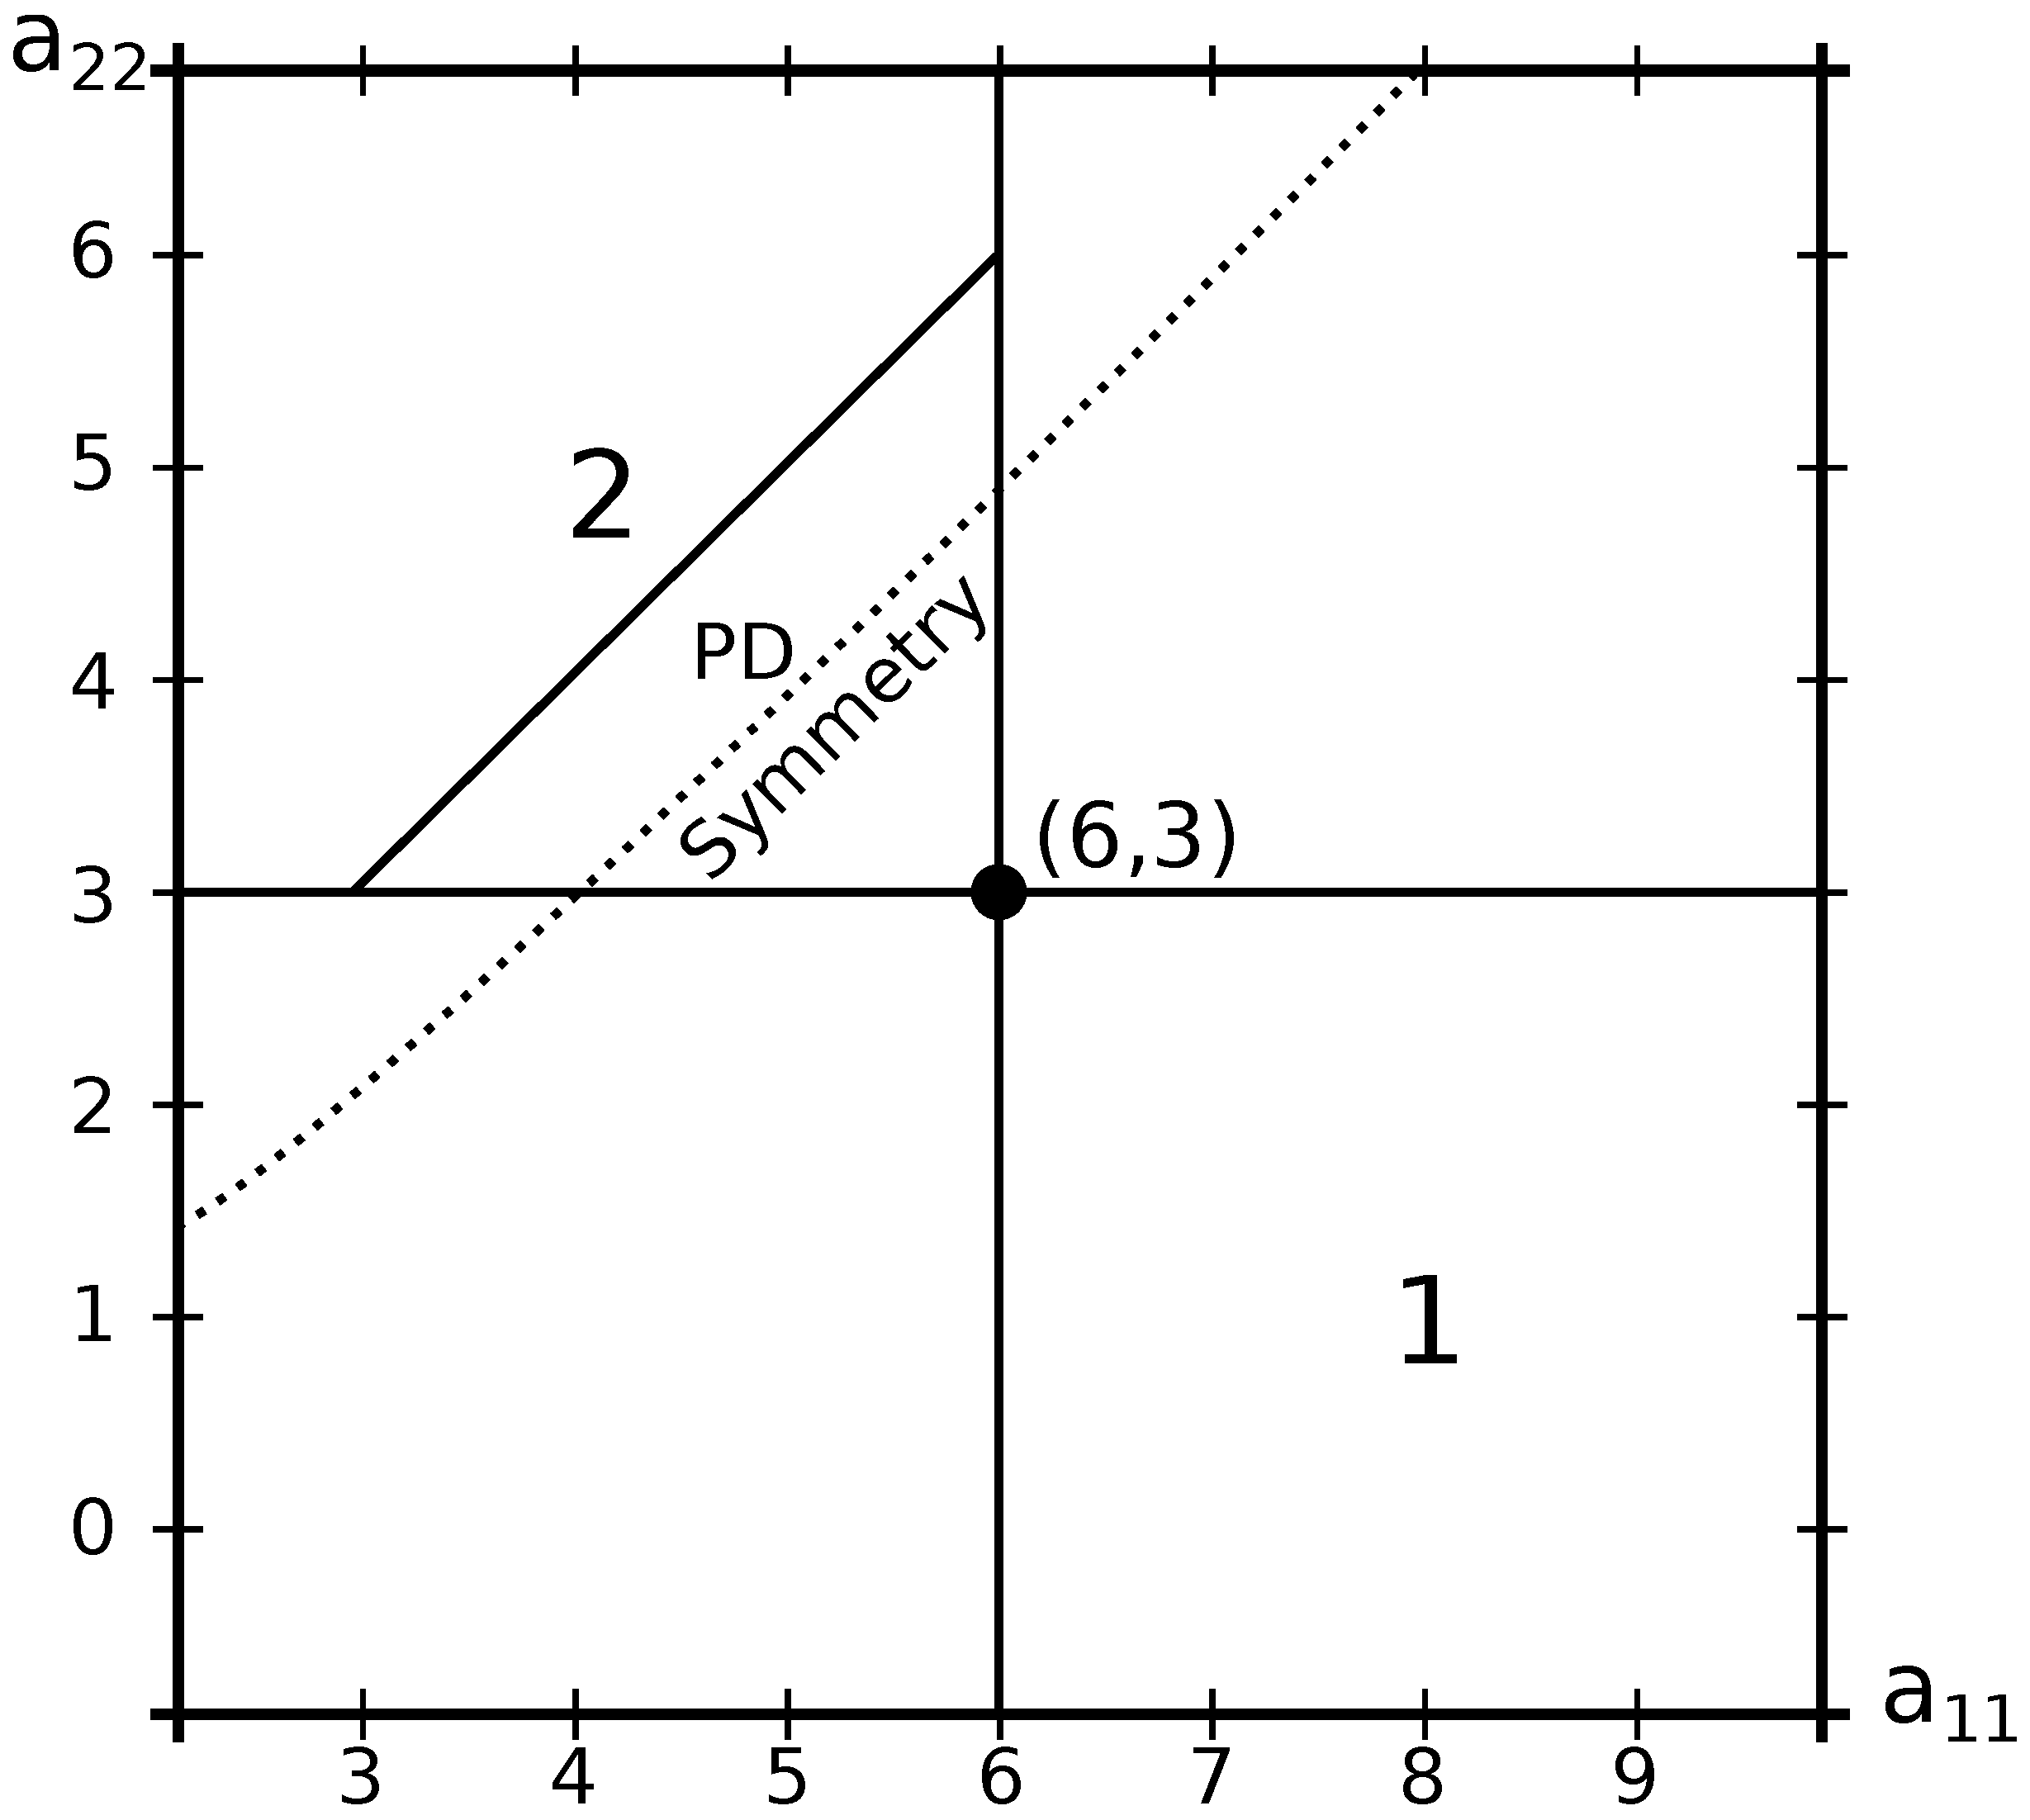
\includegraphics[width=0.6\textwidth]{./images/1d_pd_plot.eps}
\vspace{0.05\textheight}
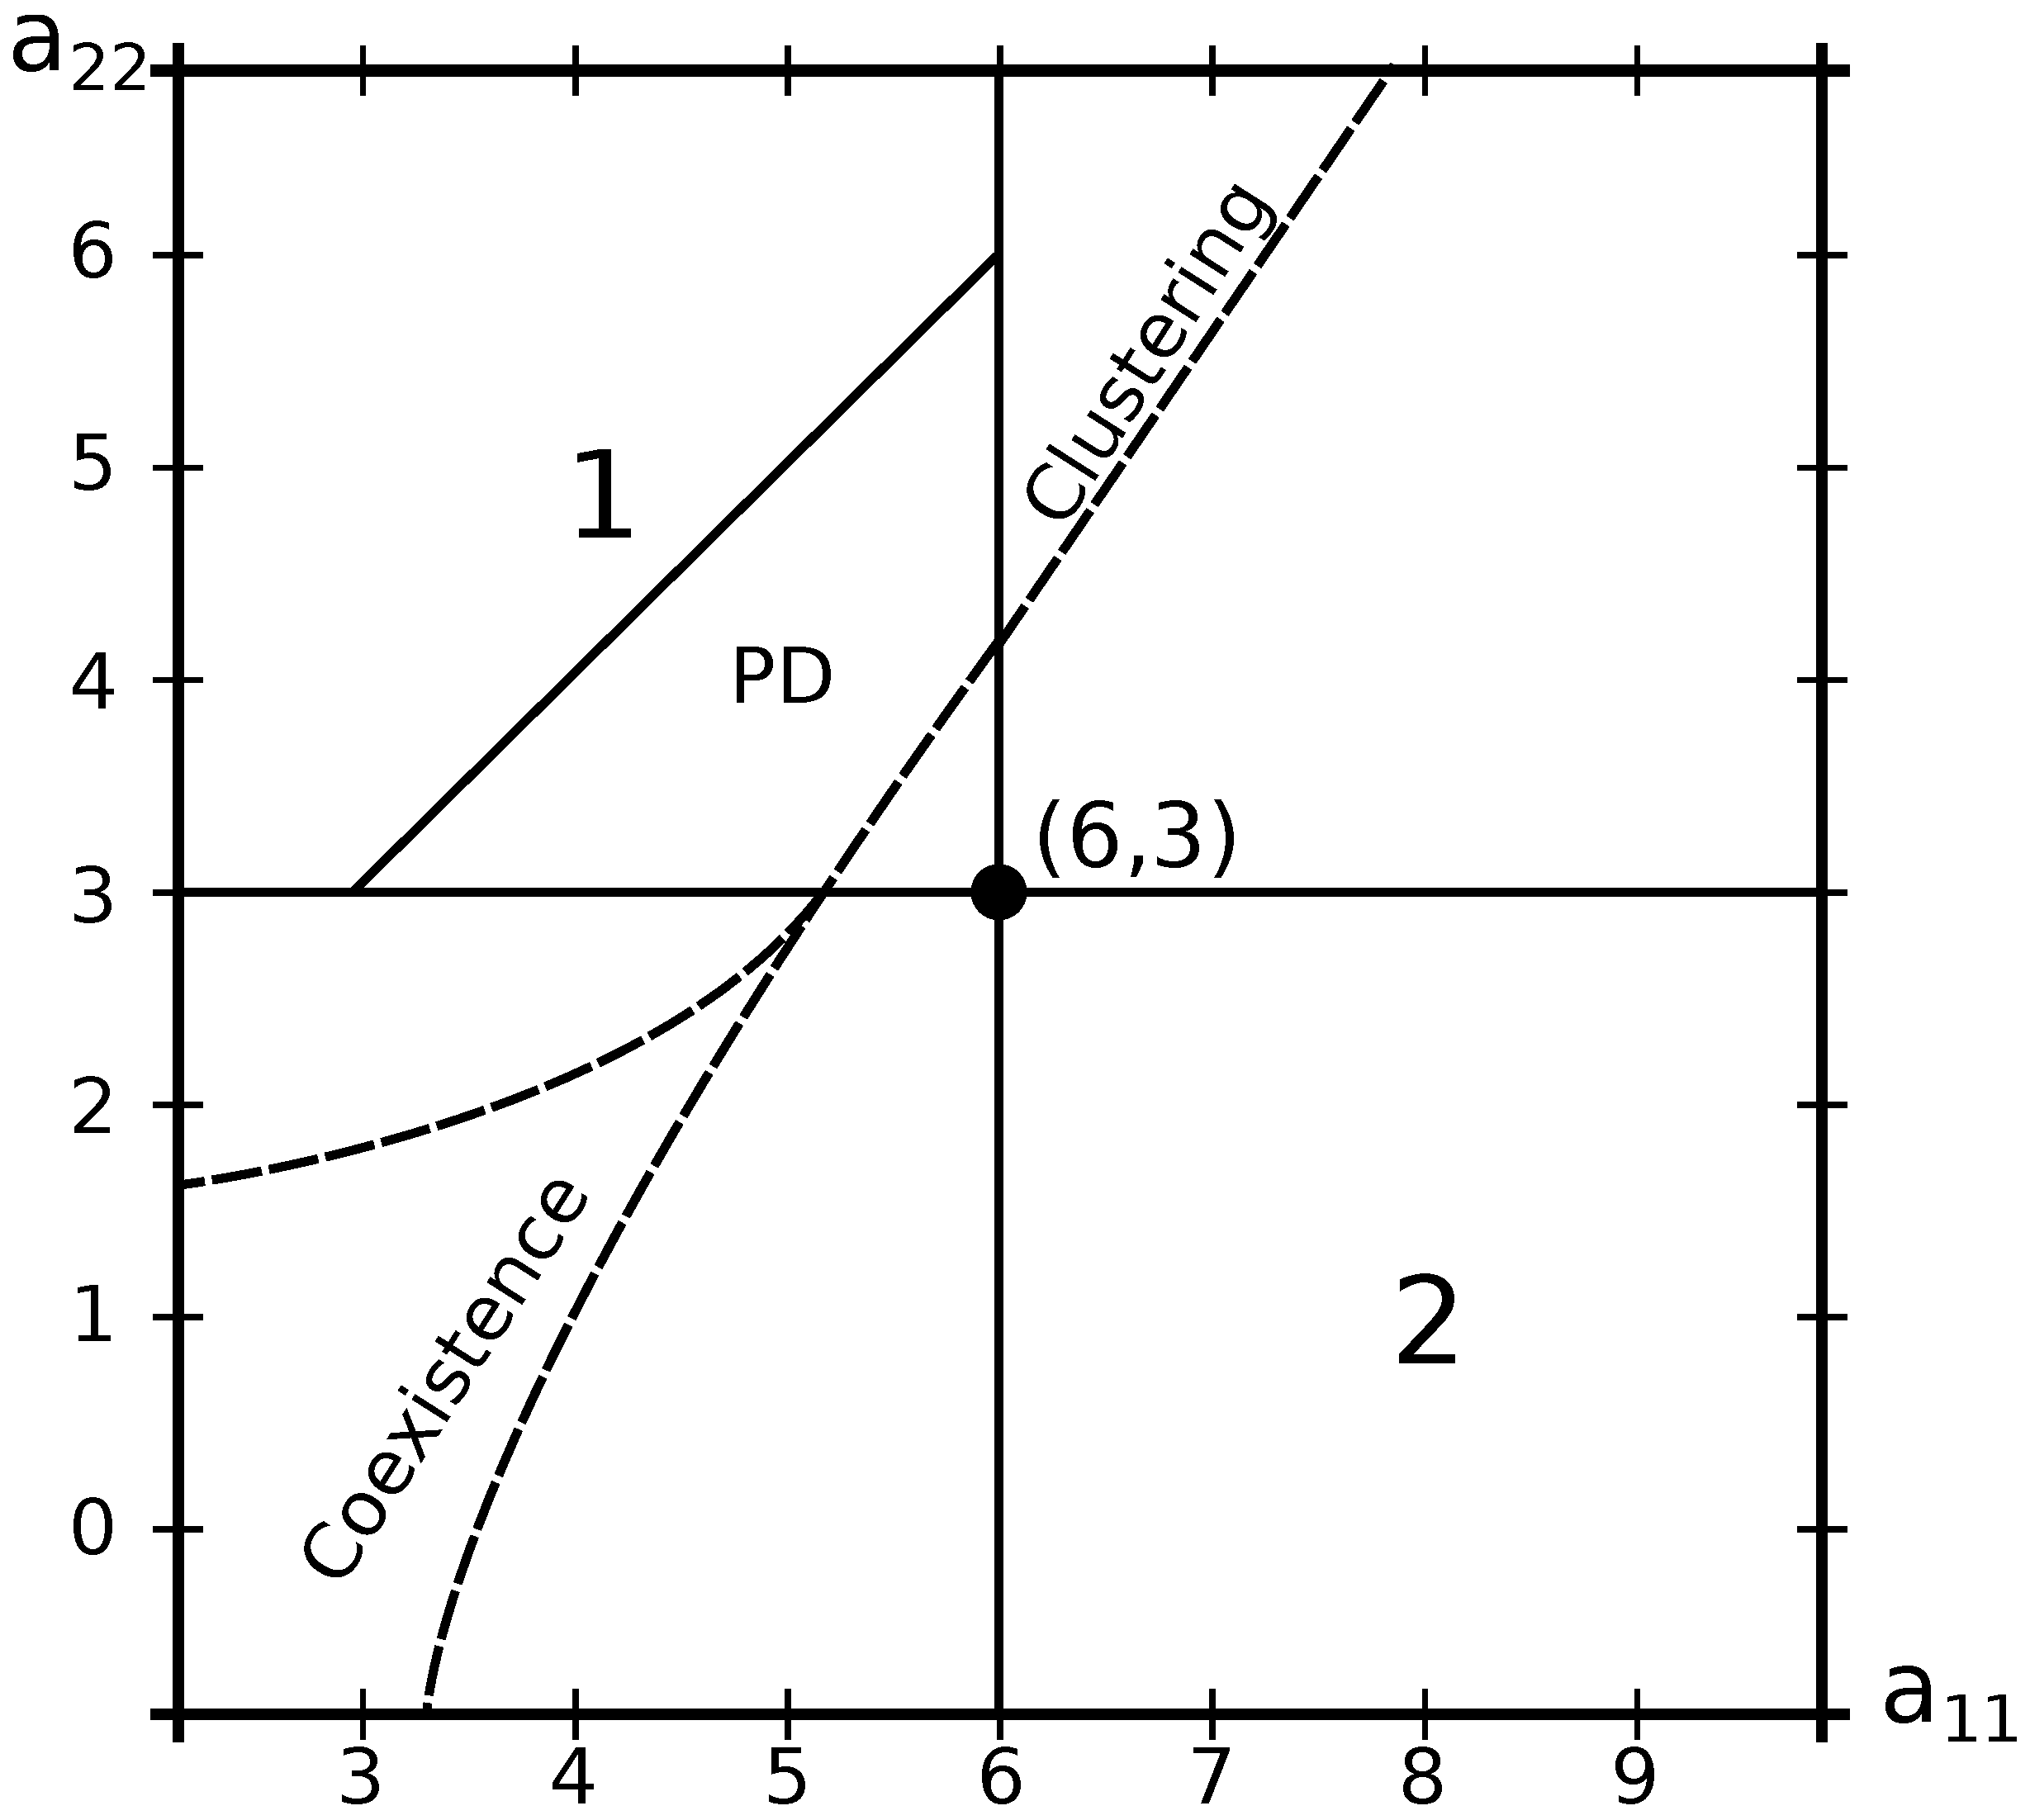
\includegraphics[width=0.6\textwidth]{./images/group_2_bifurcation_diagram_w_PD_line.eps}
    \end{figure}
  \end{column}
  \begin{column}{0.5\textwidth}
    \emph{A special case proof: continuous-time random walk}
    \begin{figure}
      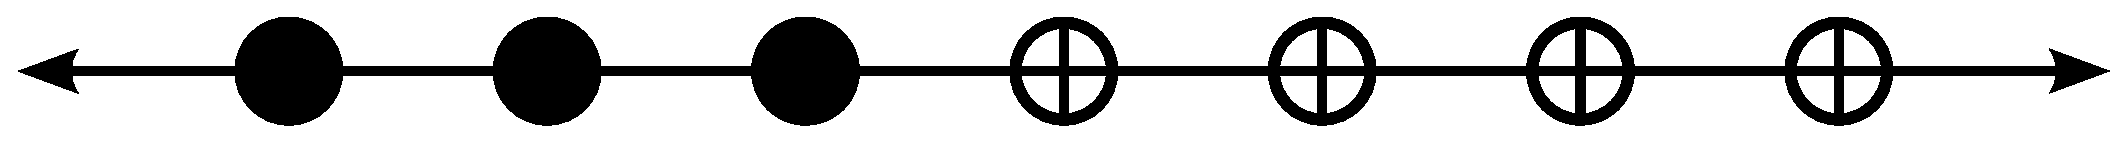
\includegraphics[width=0.7\textwidth]{./images/1dInitialConfig.eps}
    \end{figure}
The curve
\[
    a_{22}^2 + a_{22}a_{21} = a_{11}^2+a_{11}a_{12}
\]
represents a symmetric random walk for the interface. Below the curve, cooperators win.

A similar result is found in simulation.
    \begin{figure}
    \end{figure}
  \end{column}
\end{columns}
\end{frame}

\section{Acknowledgements}
\begin{frame}[c]{Acknowledgements}
Thanks for listening!

\small{Thanks also to:

My advisor, Dr. Nicolas Lanchier

Arizona State University and Barrett, the Honors College}

MAA and Pima CC for hosting.

\end{frame}

\end{document}